\documentclass[tikz]{standalone}
\usepackage{amsmath}
\usepackage{times}
\usepackage{txfonts}

\usetikzlibrary{arrows}
\usetikzlibrary{intersections}
\usetikzlibrary{math}
\usetikzlibrary{positioning}
\usetikzlibrary{arrows.meta}
\usetikzlibrary{shapes.misc}
\usetikzlibrary{calc}

\begin{document}
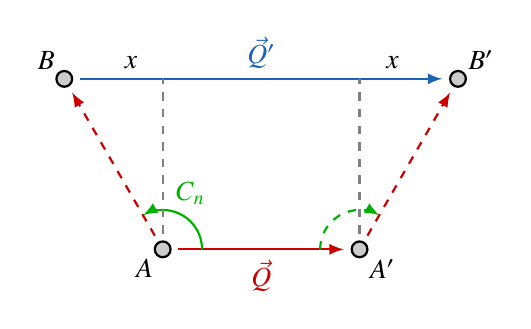
\begin{tikzpicture}[
    >=latex, 
    dot/.style = {
      draw, circle, thick, black, fill = gray!40!white,
      minimum size = 2mm,
      inner sep = 0pt,
      outer sep = 1mm,
    },
  ]

  \node[dot] (A1) at (0,0) {};
  \node[below left] at (A1) {\(A\)};

  \node[dot] (A2) at (2.5,0) {};
  \node[below right] at (A2) {\(A'\)};

  \draw[red!80!black, thick, ->] 
    (A1) to node[midway, below] {\(\vec{Q}\)} (A2);

  \node[dot] (B1) at (120:2.5) {};
  \node[above left] at (B1) {\(B\)};

  \draw[green!70!black, thick, ->]
    (A1) ++(.5,0) arc (0:120:.5)
    node[midway, above, xshift=1mm] {\(C_n\)};
  \draw[red!80!black, dashed, thick, ->] (A1) to (B1);

  \node[dot] (B2) at ($(A2)+(60:2.5)$) {};
  \node[above right] at (B2) {\(B'\)};

  \draw[green!70!black, thick, dashed, ->]
    (A2) ++(-.5,0) arc (180:60:.5);
  \draw[red!80!black, dashed, thick, ->] (A2) to (B2);

  \draw[cyan!40!blue, thick, ->]
    (B1) to node[above, midway] {\(\vec{Q}'\)} (B2);

  \draw[gray, dashed, thick] (A1) to (A1 |- B1) node (Xl) {};
  \draw[gray, dashed, thick] (A2) to (A2 |- B2) node (Xr) {};
  \node[above left, xshift=-2mm] at (Xl) {\(x\)};
  \node[above right, xshift= 2mm] at (Xr) {\(x\)};
\end{tikzpicture}
\end{document}
